\chapter{Introduction au Réseaux de Neurones}
\chapterintrobox{Les réseaux neuronaux sont des systèmes de calcul capables d'identifier les tendances dans les données et de trouver des fonctions complexes qui relient une entrée à une sortie. ces systèmes peuvent être utilisés pour une variété de tâches comme la régression et la classification. Ils peuvent être utilisés dans le domaine de la maintenance prédictive et des pronostics pour estimer l'état de santé de l'équipement et prévoir avec une certaine incertitude sa durée de vie utile restante. Ce chapitre traite les réseaux de neurones, leur topologie, leur entraînement et leur formulation mathématique.}


\section{La structure de réseaux de neurones}
Les réseaux neuronaux sont des systèmes de calcul utilisés pour trouver la correspondance entre une entrée et une sortie, ils sont constitués de plusieurs couches (couche d'entrée, couche de sortie et un nombre arbitraire de couches cachées entre l'entrée et la sortie) et chaque couche contient un certain nombre de neurones où chaque neurone de chaque couche est connecté à tous les neurones de la couche précédente et de la couche suivante (à l'exception des couches d'entrée et de sortie qui sont connectées uniquement aux couches suivante et précédente respectivement).
chaque neurone de chaque couche reçoit une entrée des neurones de la couche précédente (sous la forme d'un vecteur), multiplie le vecteur par quelques poids et somme le résultat puis applique une fonction d'activation non linéaire. Chaque neurone se retrouve avec une seule valeur numérique appelée activation, qui sera transmise aux neurones de la couche suivante.

Figure \ref{fig:neural-network-structure} montre un réseau de neurones avec la structure suivante :

\begin{itemize}
    \item Une couche d'entrée avec 3 entrée
    \item Une seule couche cachée avec 4 neurones
    \item Une couche de sortie avec 1 neurone 
\end{itemize}

\begin{figure}[h]
    \centering
	

	
		
		
\begin{tikzpicture}[neuron/.style={circle,draw, thick,align=center, minimum size=2em,inner sep=1pt}, input/.style={->}]

\node[text width=2cm, align=center] at (0,.5*\nodedist) {\small Input Layer};

\node[text width=2cm, align=center] at (\layerdist,.5*\nodedist) {\small Hidden Layer};

\node[text width=2cm, align=center] at (2*\layerdist,.5*\nodedist) {\small Output Layer};

\foreach \y in {1,...,3} \node[] (in\y) at (-\layerdist*.5,-\y*\nodedist) {$x_\y^{(i)}$};  

\foreach \y in {1,...,3} \node[neuron]  (I\y) at (0,-\y*\nodedist) {$a_\y^{[1]}$};  

\foreach \in in {1,...,3} \draw[->, >=angle 60] (in\in) --  (I\in);

\foreach \y in {1,...,4} \node[neuron]  (H\y) at ($(\layerdist,-\y*\nodedist) +(0, .5*\nodedist)$) {$a_\y^{[2]}$};

\foreach \y in {1,...,1} \node[neuron] (O\y) at ($(I2) + (2*\layerdist, 0)$) {$a_\y^{[3]}$};

\node at ($(I2) + (2.5*\layerdist, 0)$) (y) {$\hat{y}^{(i)}$};


\foreach \dest in {1,...,4} \foreach \source in {1,...,3} \draw[->, >=angle 60] (I\source) -- (H\dest);

\foreach \dest in {1,...,1} \foreach \source in {1,...,4} \draw[->, >=angle 60] (H\source) -- (O\dest);

\draw[->, >=angle 60] (O1) -- (y);

\draw[->,  thick, >=angle 60] (.5*\layerdist,-4.5*\nodedist) -- node[above] {Direction of forward propagation} (1.5*\layerdist,-4.5*\nodedist);
\draw[->,  thick, >=angle 60]  (1.5*\layerdist,-4.8*\nodedist)-- node[below] {Direction of backpropagation} (.5*\layerdist,-4.8*\nodedist);
\node [anchor=west] (note) at (-1.3*\layerdist,-4*\nodedist) {\footnotesize Single neuron};
\draw [->,  thick, >=angle 60] (note) to[out=0, in=-120] (I3.south);
\end{tikzpicture}
		
		

    \caption{Structure d'un réseau de neurones}
    \label{fig:neural-network-structure}
\end{figure}

\section{Fonction d'activation}

\subsection{L'importance des fonctions d'activation non linéaires}
L'utilisation de la fonction d'activation non linéaire est très importante pour les réseaux de neurones, ils permettent au réseau de neurones d'apprendre la correspondance non linéaire complexe de l'entrée à la sortie. Si le réseau n'utilise pas l'activation non linéaire (par exemple, l'activation linéaire ou la fonction d'identité), alors le réseau entier (quelle que soit sa profondeur) est équivalent à un réseau avec une seule couche cachée.

\subsection{Types de fonctions d'activation}
Il existe une variété de fonctions d'activation qui peuvent être utilisées pour les couches cachées et de sortie. La figure \ref{fig:activation-function} montre quelques examples:

\begin{figure}[h]
    \centering
	\documentclass[12pt]{article}
\usepackage[margin=1in]{geometry}
\usepackage{tikz}
\usetikzlibrary{arrows}
\usepackage{pgfplots}

\usepackage{caption}
\usepackage{subcaption}
\begin{document}



\begin{figure}
\begin{subfigure}[b]{0.24\linewidth}


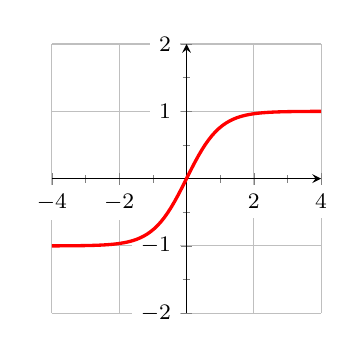
\begin{tikzpicture}
	\begin{axis}[ 
%title=$\tanh(x)$,
xmin=-4, xmax=4,ymin=-2, 
ymax=2, grid=major,
height=5cm, width=5cm,
axis line style={latex-latex},
axis lines=middle,
ticklabel style={font=\footnotesize,fill=white},
minor tick num=1,
scaled ticks=false] 
\addplot[samples=100,red,very thick] {tanh(x))};
%\addlegendentry{$\tanh(x)$}
\end{axis}
\end{tikzpicture} 
\subcaption{tanh}
\end{subfigure}
\hfill
\begin{subfigure}[b]{0.24\linewidth}



	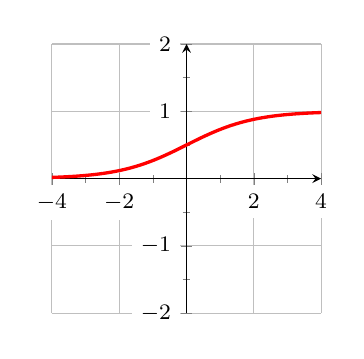
\begin{tikzpicture}
	\begin{axis}[ 
	%title=$\tanh(x)$,
	xmin=-4, xmax=4,ymin=-2, 
	ymax=2, grid=major,
	height=5cm, width=5cm,
	axis line style={latex-latex},
	axis lines=middle,
	ticklabel style={font=\footnotesize,fill=white},
	minor tick num=1,
	scaled ticks=false] 
	\addplot[samples=100,red,very thick] {1/(1+exp(-x))};
	%\addlegendentry{$\tanh(x)$}
	\end{axis}
	\end{tikzpicture}
	
	
	
\subcaption{sigmoid}
\end{subfigure}
\hfill
	\begin{subfigure}[b]{0.24\linewidth}
		
		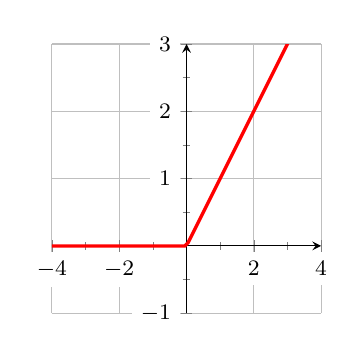
\begin{tikzpicture}
		\begin{axis}[ 
		%title=$\tanh(x)$,
		xmin=-4, xmax=4,ymin=-1, 
		ymax=3, grid=major,
		height=5cm, width=5cm,
		axis line style={latex-latex},
		axis lines=middle,
		ticklabel style={font=\footnotesize,fill=white},
		minor tick num=1,
		scaled ticks=false] 
		\addplot[samples=100,red,very thick] {max(0,x)};
		%\addlegendentry{$\tanh(x)$}
		\end{axis}
		
		\end{tikzpicture}

\subcaption{ReLU}
	\end{subfigure}
\hfill
		\begin{subfigure}[b]{0.24\linewidth}
			
		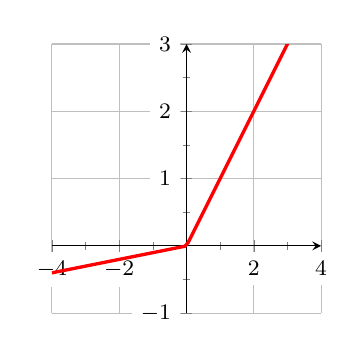
\begin{tikzpicture}
		\begin{axis}[ 
		%title=$\tanh(x)$,
		xmin=-4, xmax=4,ymin=-1, 
		ymax=3, grid=major,
		height=5cm, width=5cm,
		axis line style={latex-latex},
		axis lines=middle,
		ticklabel style={font=\footnotesize,fill=white},
		, xticklabel style={anchor=north},
		minor tick num=1,
		scaled ticks=false] 
		\addplot[samples=100,red,very thick] {max(0,x)+min(0,0.1*x)};
		%\addlegendentry{$\tanh(x)$}
		\end{axis}
		
		\end{tikzpicture}
		\subcaption{Leaky ReLU}
		\end{subfigure}
			
			\caption{Different activation functions}	

\end{figure}
\end{document}
    \caption{Différentes fonctions d'activation}
    \label{fig:activation-function}
\end{figure}


\section{Entraînement du réseau}
Le processus de formation d'un réseau de neurones consiste à déterminer les poids (coefficients) qui relient les neurones de chaque couche aux neurones de la couche suivante. Ce processus peut être formulé en termes plus mathématiques comme un problème d'optimisation : optimisation des coefficients du réseau pour trouver leurs valeurs qui minimisent une fonction de coût.

L'entraînement du réseau de neurones utilise des données d'entraînement (training data) qui fournissent des entrées et leurs sorties correspondantes.

\subsection{Fonction de coût}


\subsection{Backpropagation}
\begin{figure}[h]
    \centering
	\documentclass[12pt]{article}
\usepackage{tikz}
\usetikzlibrary{arrows,positioning}
\begin{document}
	

\begin{tikzpicture}[arrow/.style={thick, >=angle 60}]
	\node[draw, circle,thick,minimum width=3em, inner sep=0] (fp) {\large $f(x)$};
	\node[above left = 2em of fp] (x1) {\large $x_1$};
	\node[below left = 2em of fp] (x2) {\large $x_2$};
	\node[right = 2em of fp] (y1) {\large $y_1$};
	
	\node[above = 4em of fp] {\large Forward pass};
	
	\draw[->,arrow] (x1) -- (fp);
	\draw[->,arrow] (x2) -- (fp);
	\draw[->,arrow] (fp) -- (y1);

\node[draw, circle,thick,minimum width=2.7em, inner sep=0, right = 15 em of fp] (bp) {\large $df$};
\node[above left = 2em of bp] (bx1) {\large $\frac{\partial L}{\partial x_1}=\frac{\partial L}{\partial y_1}\frac{\partial y_1}{\partial x_1}$};

\node[below left = 2em of bp] (bx2) {\large $\frac{\partial L}{\partial x_2}=\frac{\partial L}{\partial y_1}\frac{\partial y_1}{\partial x_2}$};

\node[right = 2em of bp] (by1) {\large $\frac{\partial L}{\partial y_1}$};

\node[above = 4em of bp] {\large Backward pass};

\draw[<-,arrow] (bx1) -- (bp);
\draw[<-,arrow] (bx2) -- (bp);
\draw[<-,arrow] (bp) -- (by1);
\end{tikzpicture}
	
\end{document}
    \caption{Forward et Backward passes}
    \label{fig:forward-backward-pass}
\end{figure}



\begin{comment}
    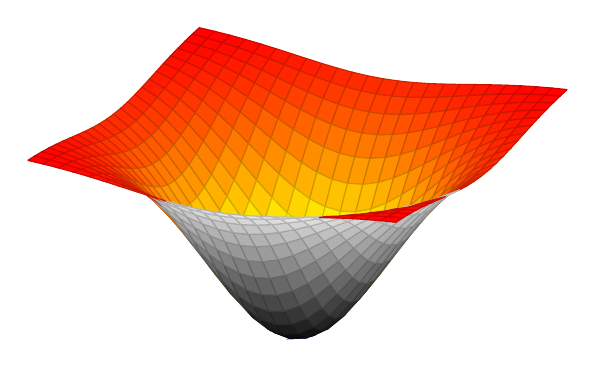
\begin{tikzpicture}
    \begin{axis}[
    hide axis,
    xlabel=$x$,ylabel=$y$,
    mesh/interior colormap name=hot,
    colormap/blackwhite,
    ]
    \addplot3 [domain=-1.5:1.5,surf]
    {-exp(-x^2-y^2)};
    \end{axis}
    \end{tikzpicture}

    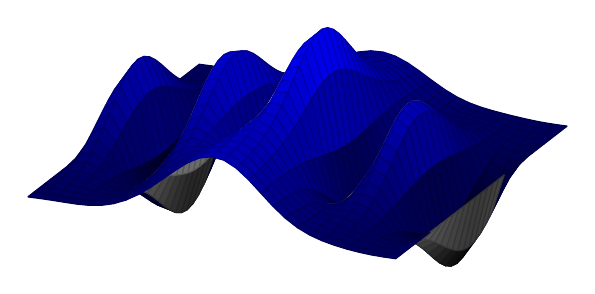
\begin{tikzpicture}
        \begin{axis}[
        hide axis,
        xlabel=$x$,
        ylabel=$y$,
        ]
        \addplot3 [
        surf,
        mesh/interior colormap={blueblack}{
        color=(black) color=(blue)
        },
        % slightly increase sampling quality (was 25):
        samples=31,
        % avoids overshooting corners:
        miter limit=1,
        % move boundary between inner and outer:
        mesh/interior colormap thresh=0.1,
        colormap/blackwhite,
        domain=0:1,
        ] {
        sin(deg(8*pi*x))* exp(-20*(y-0.5)^2)
        + exp(-(x-0.5)^2*30
        - (y-0.25)^2 - (x-0.5)*(y-0.25))
        };
        \end{axis}
        \end{tikzpicture}
\end{comment}